The solution architecture is based on the suggested architecture in Figure 4.1 of the compendium~\cite[p.115]{compendium}.
In order to support a larger instruction set, the solution architecture has been expanded somewhat.
The main differences are that the ALU control unit and the main control unit have been merged, and that a branch controller has been added to take care of branching logic.
The architecture of the presented solution processor is illustrated in figure \vref{figure:cpu-architecture}.

In figure \vref{figure:cpu-architecture}, each box corresponds to an architecture component.
Larger components have their names written the top of each box.
Smaller components have hovering labels showing their names.
The left side of a box is used for input signals, and the right side of the box is used for output signals.
The exception to this rule are the muxes, which use a variant of the classic pill-style mux diagrams: Input signals come through the top and bottom, the control signal comes in on the middle left and the output is on the middle right.

\begin{figure}[h!]
	\begin{center}
		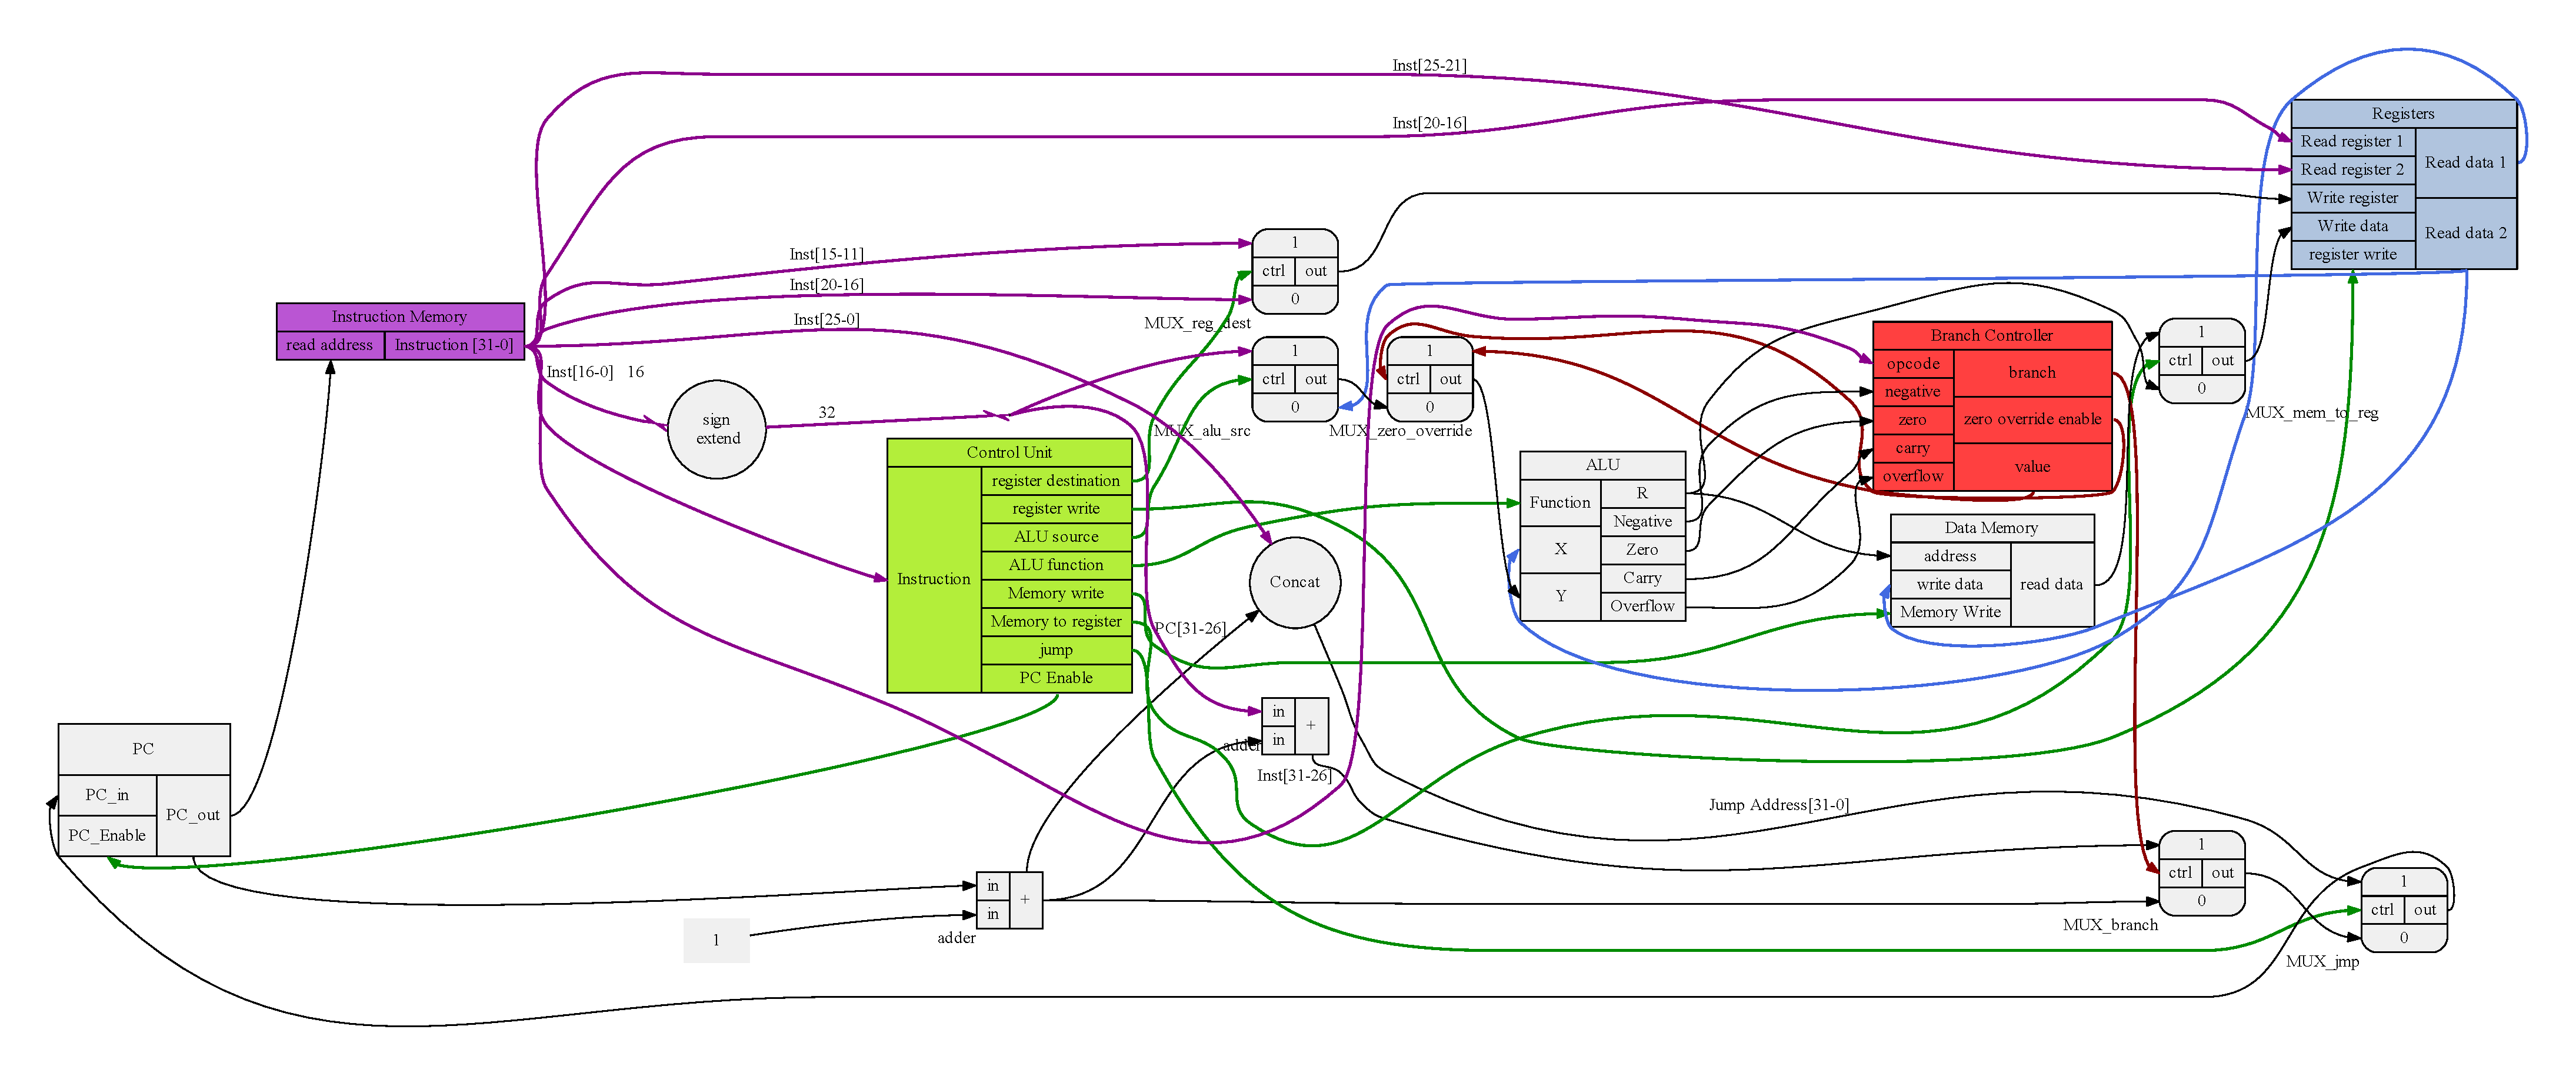
\includegraphics[keepaspectratio, height=\textheight, width=\textwidth]{graphics/cpu-architecture/cpu-architecture-color.pdf}
		\caption{Architecture of the solution processor.}
		\label{figure:cpu-architecture}
	\end{center}
\end{figure}

\subsection{ALU}

\todo{The ALU description}

\subsubsection{In Signals}

\begin{description}
\item{\textbf{Signal}} \\
Description of it.

\end{description}

\subsubsection{Out Signals}

\begin{description}
\item{\textbf{Signal}} \\
Description of it.
\end{description}


\subsection{Branch Controller}

The branch controller the logic unit that decides whether or not the program should branch.
It is separate from the main control unit, as it works independently from the control unit state machine, and does not need to follow the clock.
The branch controller reads the opcode field from the current instruction, looking for branch instructions.
If it finds a branch instruction, it will apply the logic that is required for that instruction.

Having branch logic contained in a separate branch controller gives the opportunity to implement many different branch instructions in a modular manner.

To handle the simplest operations that compare two registers to each other, the branch controller can simply look at the flags from the ALU to decide if the branch MUX should be enabled.
Instructions that compare a register to zero require a bit more work from the branch controller.
The branch controller can send out a zero value that overrides the ALU's source for the $ y $ operand, and is compared to the $ x $ operand from the register specified in the instruction.

To allow for other compare operations than $x \geq 0$ and $x < 0$, the zero value will not always be zero. 
Because the solution processor only handles integers, the comparison $ x \geq 1 $ is equivalent with $ x > 0 $.
This trick means that support for branch operations other than zero and negative are not needed, which nicely reduces complexity in the design without sacrificing performance.
Therefore the zero value from the branch controller vary from -1 to 1.

The control unit drives the branch controller by instructing the ALU to do a subtraction on its inputs, $ x - y $, and ignore the result.
This sets the zero flag of the ALU if the x = y, and the negative flag of the ALU if the x < y.
It is these flags that is used by the branch controller to detemin if it should branch.

\subsubsection{In Signals}

\begin{description}
\item{\textbf{Flags}} \\

The Flags signal comes directly from the ALU, and it tells the branch controller the outcome of a compare comparison.

\item{\textbf{Opcode}} \\

The Opcode signal, which comes directly from the currently executing instruction word, tells the branch controller what kind of branch should be checked for, if any.

\end{description}

\subsubsection{Out Signals}

\begin{description}
\item{\textbf{Compare Zero Value}} \\

TODO: rune must say what this is.

\item{\textbf{Compare Zero}} \\

TODO: rune must say what this is.

\item{\textbf{Branch}} \\

If the branch controller finally decides that a branch should be taken, the Branch signal wil be set.

\end{description}


\subsection{Control Unit}

The control unit is the component that is responsible for enabling and disabling the correct parts of the processor at the correct times, so that an instruction is executed correctly.

\subsubsection{In Signals}

\begin{description}
\item{\textbf{Instruction Op-code}} \\
    The op-code of the currently executing instruction in the instruction decode stage.

\item{\textbf{Instruction Function}} \\
    The ALU function of the currently executing instruction in the instruction decode stage. 
\end{description}

\subsubsection{Out Signals}

\begin{description}
\item{\textbf{Execute Control Signals}} \\
    The control signals that should be used in the execute stage for the instruction being decoded by the control unit.
    The execute control signals bus contains the \textbf{ALU Source}, \textbf{ALU Function} and \textbf{Register Destination} control signals.

\item{\textbf{Memory Control Signals}} \\
    The control signals that should be used in the memory stage for the instruction being decoded by the control unit.
    The memory control signals bus contains the \textbf{Branch} and \textbf{Memory Write} control signals.

\item{\textbf{Write-Back Control Signals}} \\
    The control signals that should be used in the write-back stage for the instruction being decoded by the control unit.
The write-back control signals bus contains the \textbf{Memory to Register} and \textbf{Register Write} control signals.

\item{\textbf{Jump}} \\
    Whether or not the instruction being decoded is a jumping instruction (i.e. \texttt{JMP}).
\end{description}



\subsection{Program Counter Circuit}

The program counter circuit is the loop the program counter forms together with the branch and jump circuitry.
The program counter is a register that holds the address of the next instruction to be fetched.
When no branching or jumping is involved (the ``sunny day scenario''), the program counter cycle increments the program counter by one every time the control unit tells it to.
This means that the control unit has the opportunity to advance the running program.
The control unit advances the program counter when it is in the execute state, so that a new program counter value is ready for when the control unit enters the fetch state.

When the control unit gives the signal, the program counter may perform a branch or a jump by manipulating the program counter circuit to change the value sent back to the program counter.

TODO: diagram of the program counter cycle.

\subsubsection{Program Counter}

The program counter is implemented as a D-type flip-flop with reset and enable signals.

\subsubsubsection{In Signals}

\begin{description}
\item{\textbf{Clock}} \\

Clock.

\item{\textbf{Program Counter In}} \\

On rising edge, of the clock, the program counter's new value is fetched from this signal.

\item{\textbf{Reset}} \\

When the reset signal is high, the program counter is reset to 0 on the next rising edge of the clock.

\end{description}

\subsubsubsection{Out Signals}

\begin{description}
\item{\textbf{Program Counter Out}} \\

This signal is set to the current value of the program counter.

\end{description}

TODO: explain other parts of this thing?


\subsection{Multiplexer}

The multiplexer is a simple, ordinary multiplexer implemented as a VHDL entity for tidiness and modularity.
Although quite trivial, it is documented here for completeness.

\subsubsection{In Signals}

\begin{description}
\item{\textbf{Input 0}} \\
A generic \texttt{std\_logic\_vector} input.

\item{\textbf{Input 1}} \\
A generic \texttt{std\_logic\_vector} input.

\item{\textbf{Selector}} \\
A boolean select signal that selects either Input 0 or Input 1 to be passed on as output.
In the architecture diagram these are labeled as ``\texttt{ctrl}''. 
In the VHDL code it is the ``\texttt{enable}'' signal.

\end{description}

\subsubsection{Out Signals}

\begin{description}
\item{\textbf{Output}} \\
Input 0 or Input 1, decided by the Selector.
\end{description}

